\documentclass{article}
\usepackage[paperwidth=338.67mm,paperheight=190.5mm,margin=13mm]{geometry}
\usepackage{fontspec,graphicx,xcolor,booktabs,tabularx,tikz,hyperref}
\setsansfont{Calibri}\renewcommand{\familydefault}{\sfdefault}
\definecolor{Ink}{HTML}{173047}\definecolor{Ember}{HTML}{BC4221}\definecolor{Mist}{HTML}{EEF4F7}\definecolor{Muted}{HTML}{536575}
\pagecolor{Mist}\color{Ink}\pagestyle{empty}\setlength{\parindent}{0pt}\setlength{\parskip}{4mm}
\hypersetup{colorlinks=true,urlcolor=Ember,pdfauthor={Team KUETaguns},pdftitle={Agun Panjika: global demo in seven slides}}
\newcommand{\kicker}[1]{{\fontsize{11}{14}\selectfont\color{Ember}\MakeUppercase{#1}}\par}
\newcommand{\headline}[1]{{\fontsize{32}{35}\selectfont\bfseries #1}\par\vspace{4mm}}
\newcommand{\smallnote}[1]{{\fontsize{11}{14}\selectfont\color{Muted}#1}\par}
\newcommand{\footer}[2]{\begin{tikzpicture}[remember picture,overlay]\node[anchor=south west,font=\fontsize{9}{11}\selectfont,text=Muted] at ([xshift=13mm,yshift=6mm]current page.south west){#1};\node[anchor=south east,font=\fontsize{10}{12}\selectfont,text=Muted] at ([xshift=-13mm,yshift=6mm]current page.south east){#2 / 7};\end{tikzpicture}}
\newcommand{\CountryCount}{242}
\newcommand{\CaseTableRows}{Bangladesh & 46.9 & 58.3 & 78.2\% \\
Nepal & 115.2 & 158.5 & 79.6\% \\
Chin, Myanmar & 88.5 & 97.3 & 74.6\% \\
Punjab \& Haryana, India & 246.3 & 262.0 & 82.4\% \\}

\begin{document}\fontsize{20}{26}\selectfont\raggedright
\kicker{Team KUETaguns · NASA Space Apps Challenge 2026}
\begin{minipage}[t]{.38\linewidth}\vspace{0pt}\headline{Agun Panjika}
{\fontsize{25}{29}\selectfont A fire history you can inspect.}\par
\vspace{4mm}\smallnote{Harmonization of MODIS and VIIRS Hot Spots}
\vspace{4mm}\smallnote{Worldwide observations.\newline Evaluated historical calendars.\newline Evidence you can explore and share.}
\end{minipage}\hfill\begin{minipage}[t]{.59\linewidth}\vspace{0pt}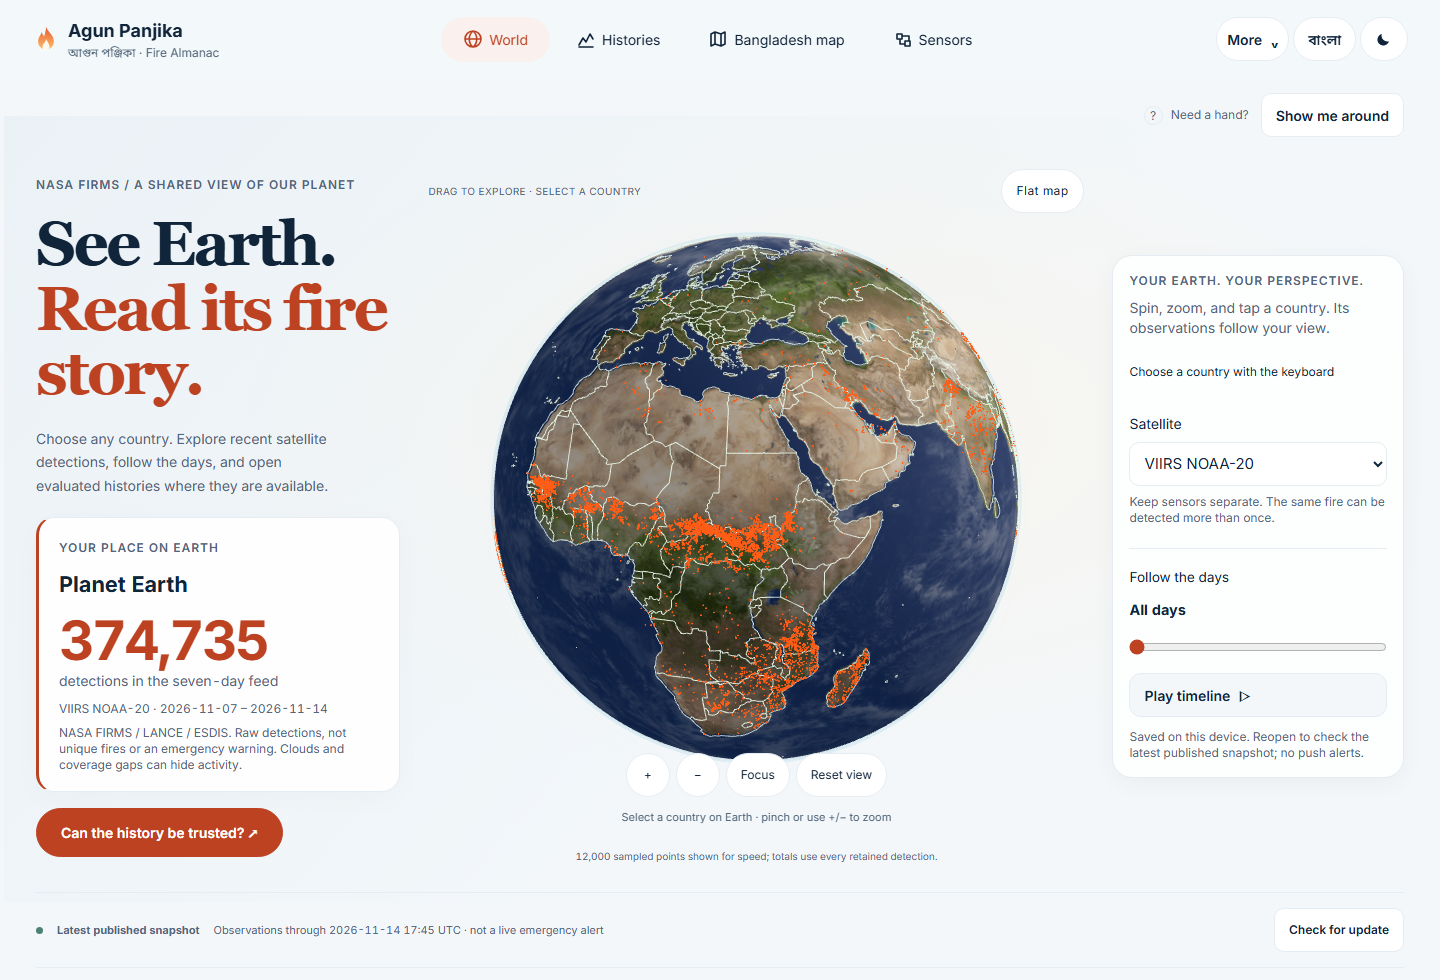
\includegraphics[width=\linewidth]{../review/screenshots/world-hero.png}\end{minipage}
\vspace{5mm}
{\fontsize{13}{17}\selectfont Sohaib Hasan Niloy · Ayesha Mehereen · Sarwad Hasan Siddiqui\par Adiba Tahsin · Abdullah Al Saif · Md. Rafsani Shazid}
\footer{Actual application capture · 15 November 2026}{1}

\newpage\kicker{The opportunity}\headline{Bring satellite records together.}
\begin{minipage}[t]{.64\linewidth}\vspace{0pt}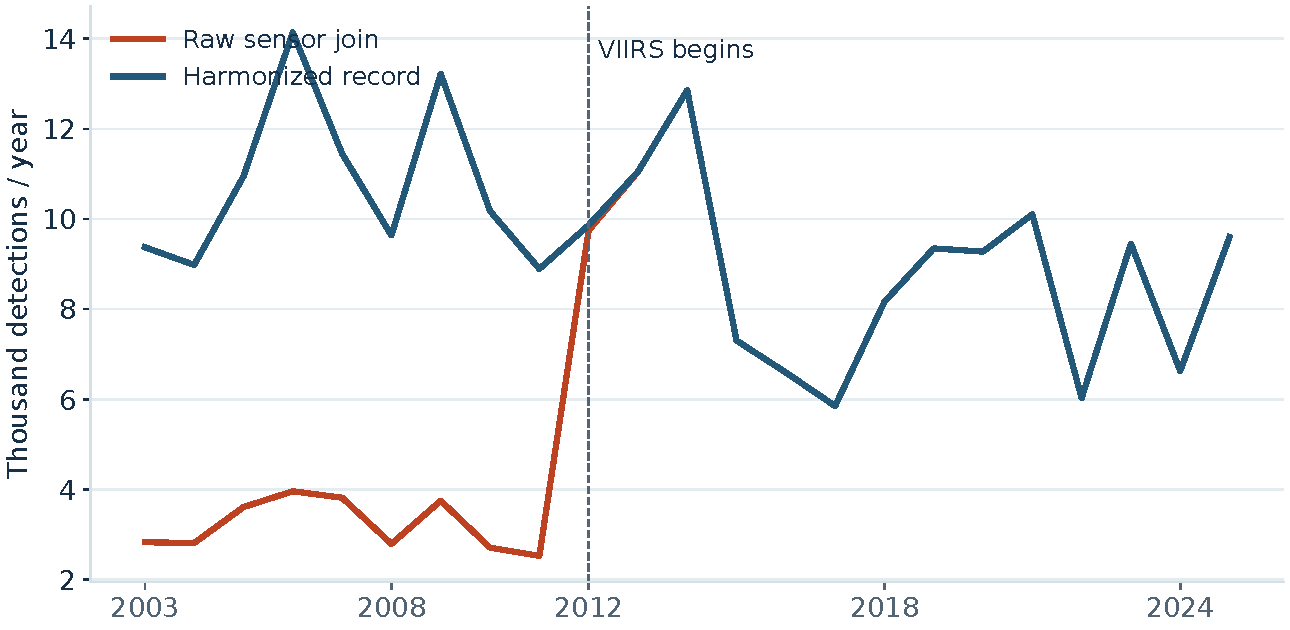
\includegraphics[width=\linewidth,height=108mm,keepaspectratio]{../latex/figures/sensor-story.pdf}\end{minipage}\hfill
\begin{minipage}[t]{.31\linewidth}\vspace{0pt}
\textbf{MODIS: about 1 km.}\par\textbf{VIIRS: 375 m.}\par\vspace{3mm}
{\fontsize{18}{23}\selectfont Connecting these observations helps people explore fire seasons across a change in satellite instruments.}\par
\vspace{3mm}\smallnote{Satellite detection counts · Bangladesh historical example · seasonal and sensor variation.}
\end{minipage}
\footer{NASA FIRMS · Bangladesh example · AI-assisted plotting of project exports}{2}

\newpage\kicker{The solution}\headline{Explore the present. Inspect the past.}
\begin{minipage}[t]{.31\linewidth}\vspace{0pt}{\color{Ember}\fontsize{38}{40}\selectfont 01}\par\textbf{Choose a place.}\par{\fontsize{18}{23}\selectfont Spin the Earth and tap a country. Separate MODIS, NOAA-20 and NOAA-21 views show recent observations.}\end{minipage}\hfill
\begin{minipage}[t]{.31\linewidth}\vspace{0pt}{\color{Ember}\fontsize{38}{40}\selectfont 02}\par\textbf{Check the record.}\par{\fontsize{18}{23}\selectfont In an evaluated area, compare a raw sensor join, a fitted factor and a reconstruction against withheld VIIRS.}\end{minipage}\hfill
\begin{minipage}[t]{.31\linewidth}\vspace{0pt}{\color{Ember}\fontsize{38}{40}\selectfont 03}\par\textbf{Keep the evidence.}\par{\fontsize{18}{23}\selectfont Export dates, source, uncertainty and limits together. Return to a saved country on your phone.}\end{minipage}
\par\vspace{9mm}\smallnote{Recent observations in \CountryCount{} countries and territories. Historical reconstruction evaluated in Bangladesh, Nepal, Chin and Punjab--Haryana.}
\footer{NASA FIRMS / LANCE / ESDIS · Three.js · React · D3 · static exports}{3}

\newpage\kicker{Measured progress}\headline{Better estimates for major fire seasons.}
\begin{minipage}[t]{.64\linewidth}\vspace{0pt}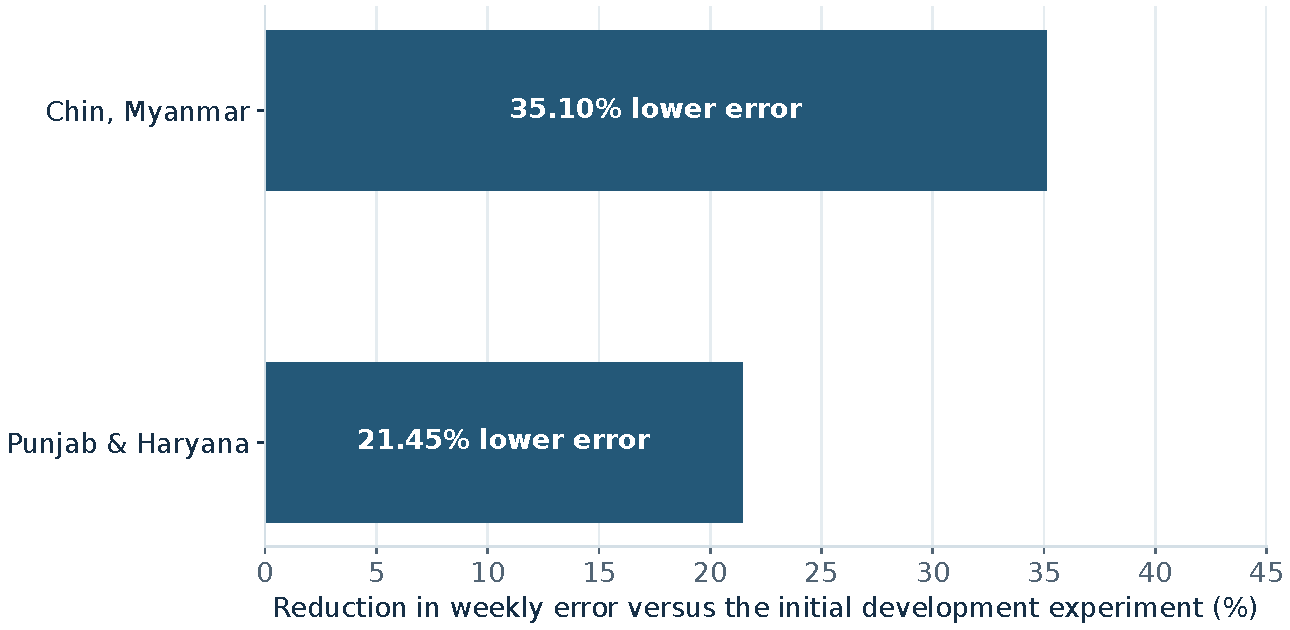
\includegraphics[width=\linewidth,height=105mm,keepaspectratio]{../latex/figures/global-impact.pdf}\end{minipage}\hfill
\begin{minipage}[t]{.31\linewidth}\vspace{0pt}{\fontsize{17}{22}\selectfont
\textbf{Chin:} better capture an exceptional seasonal peak.\par\vspace{3mm}
\textbf{Punjab--Haryana:} keep estimates responsive with annual past-only updates.}\par
\vspace{5mm}\smallnote{Weekly mean absolute error versus the previous release. Historical replay, 2022--2024: all 156 original weeks per area. Complete four-area comparisons in the linked model card.}
\end{minipage}
\footer{Source: versioned project evaluations · reproducible from public feature files}{4}

\newpage\kicker{The experience}\headline{See the correction in action.}
\begin{minipage}[t]{.75\linewidth}\vspace{0pt}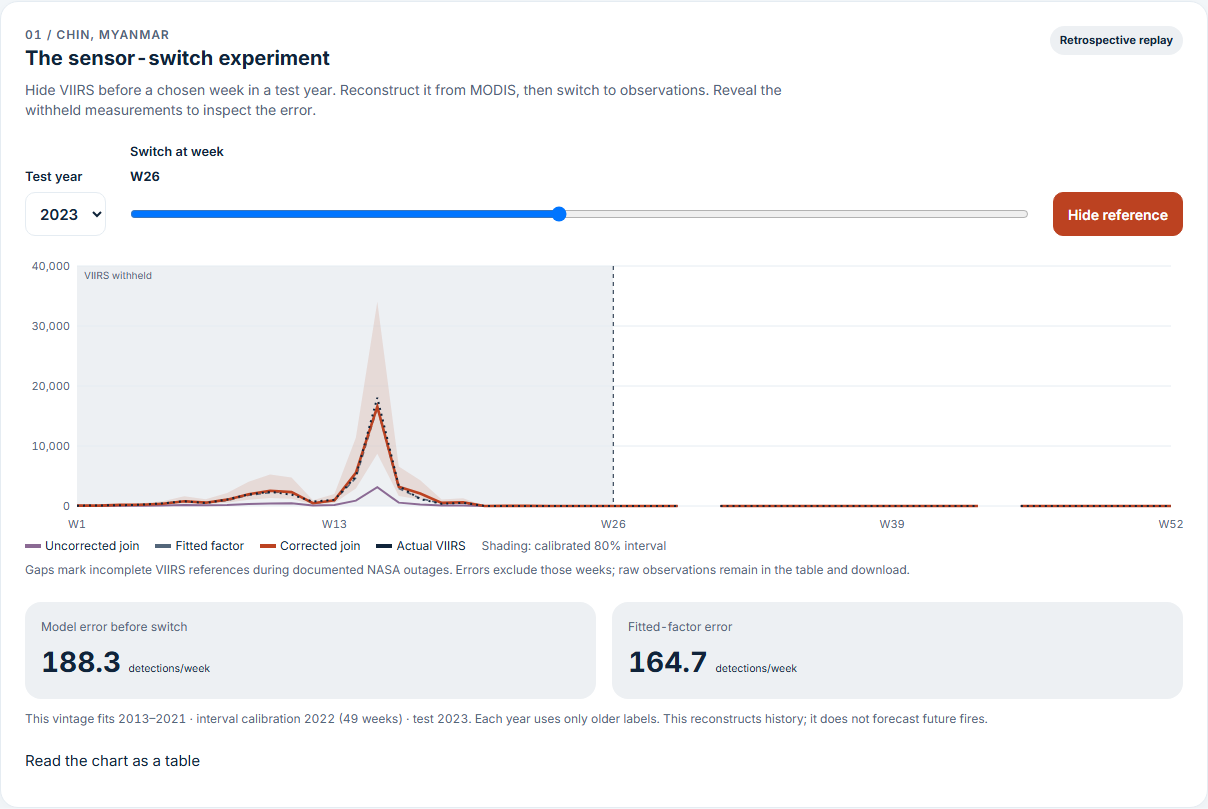
\includegraphics[width=\linewidth,height=109mm,keepaspectratio]{../review/screenshots/global-experiment.png}\end{minipage}\hfill
\begin{minipage}[t]{.21\linewidth}\vspace{0pt}{\fontsize{18}{24}\selectfont Choose a season.\par Move the switch week.\par Reveal VIIRS.\par Compare the curves.}\vspace{5mm}\smallnote{Past-only model vintages, interval bounds, source dates and accessible data tables.}
\end{minipage}
\footer{Actual application capture · historical reconstruction with a revealable satellite reference}{5}

\newpage\kicker{Intended impact}\headline{Check your country on your phone.}
\begin{minipage}[t]{.27\linewidth}\vspace{0pt}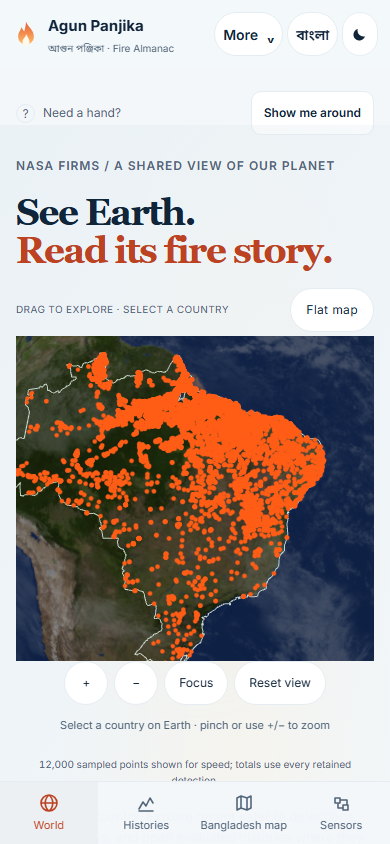
\includegraphics[height=117mm,width=\linewidth,keepaspectratio]{../review/screenshots/world-phone.png}\end{minipage}\hfill
\begin{minipage}[t]{.68\linewidth}\vspace{0pt}{\fontsize{20}{26}\selectfont
\textbf{For a student:} investigate observations in their own country.\par\vspace{3mm}
\textbf{For a local group:} share a dated observation brief with its source.\par\vspace{3mm}
\textbf{For researchers and land managers:} inspect seasonal patterns and periods worth monitoring.}\par\vspace{4mm}
\smallnote{Eight-step guided tutorial · installable PWA · local watchlist · offline reference data · keyboard/flat-map alternatives · reduced motion.}\par
\smallnote{Designed to support learning, community discussion and research into seasonal fire activity.}
\end{minipage}
\footer{Actual mobile capture · cached data retains its observation date}{6}

\newpage\kicker{Team KUETaguns}\headline{Try the app and check the evidence.}
\begin{minipage}[t]{.58\linewidth}\vspace{0pt}{\fontsize{22}{28}\selectfont\href{https://polymathicx.github.io/Agun-Panjika/}{Open the application}\par\href{https://github.com/polymathicX/Agun-Panjika}{Code, model card and reproducible results}}\par\vspace{5mm}
{\fontsize{16}{21}\selectfont Sohaib Hasan Niloy · Ayesha Mehereen\par Sarwad Hasan Siddiqui · Adiba Tahsin\par Abdullah Al Saif · Md. Rafsani Shazid}\par\vspace{4mm}\smallnote{Challenge: Harmonization of MODIS and VIIRS Hot Spots}
\end{minipage}\hfill\begin{minipage}[t]{.37\linewidth}\vspace{0pt}
\smallnote{\textbf{Data:} NASA FIRMS / LANCE / ESDIS. NASA POWER and ESA Fire\_cci support the Bangladesh research pipeline.}\par
\smallnote{\textbf{Geography and imagery:} geoBoundaries; Natural Earth; Solar System Scope textures, CC BY 4.0. Earth/cloud imagery provides geographic context.}\par
\smallnote{\textbf{Assistance:} AI helped coding, review, plotting, documentation and demo assembly. Raw observations are NASA measurements; model outputs are labeled estimates.}\par
\smallnote{Original code: Apache 2.0; third-party terms retained. Independent NASA Space Apps team project.}
\end{minipage}
\footer{15 November 2026 · review the full project page and source artifacts}{7}
\end{document}
